\documentclass[tikz,border=8pt]{standalone}
\usepackage{amsmath}
\usepackage{amssymb}
\usetikzlibrary{arrows.meta,positioning,fit,calc}

\begin{document}
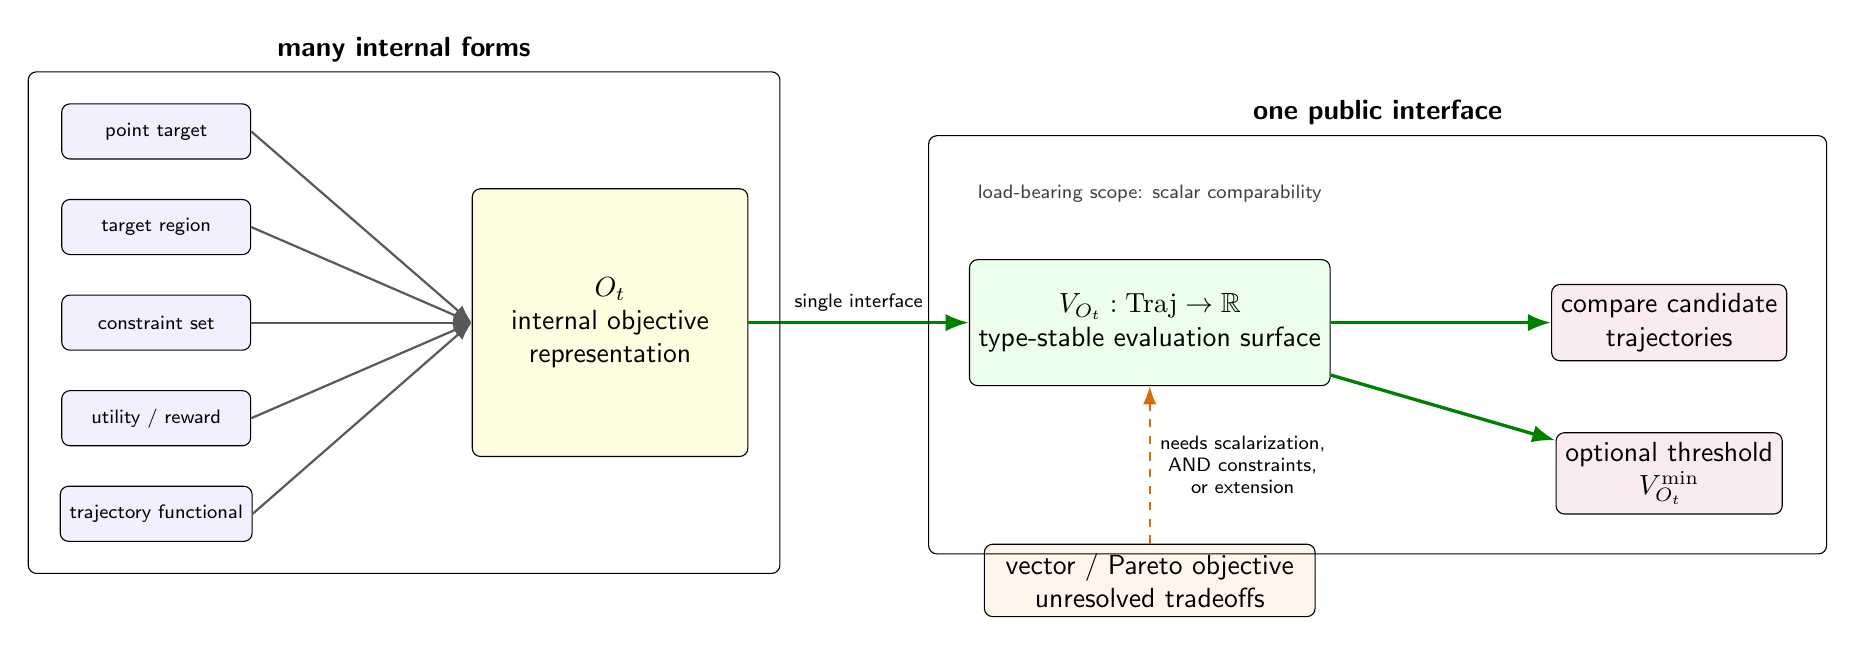
\begin{tikzpicture}[
  font=\sffamily,
  box/.style={draw, rounded corners=3pt, align=center, minimum width=28mm, minimum height=8mm, fill=white},
  small/.style={draw, rounded corners=3pt, align=center, minimum width=24mm, minimum height=7mm, fill=white, font=\sffamily\scriptsize},
  arrow/.style={-Latex, thick, draw=black!65},
  good/.style={-Latex, very thick, draw=green!50!black},
  warn/.style={-Latex, thick, dashed, draw=orange!85!black},
  note/.style={align=center, font=\sffamily\scriptsize}
]

\node[small, fill=blue!6] (target) {point target};
\node[small, below=5mm of target, fill=blue!6] (region) {target region};
\node[small, below=5mm of region, fill=blue!6] (constraint) {constraint set};
\node[small, below=5mm of constraint, fill=blue!6] (utility) {utility / reward};
\node[small, below=5mm of utility, fill=blue!6] (trajfun) {trajectory functional};

\node[box, right=28mm of constraint, fill=yellow!12, minimum width=35mm, minimum height=34mm] (objective)
  {$O_t$\\internal objective\\representation};

\node[box, right=28mm of objective, fill=green!8, minimum width=42mm, minimum height=16mm] (value)
  {$V_{O_t}:\mathrm{Traj}\to\mathbb{R}$\\type-stable evaluation surface};

\node[box, right=28mm of value, fill=purple!8] (compare)
  {compare candidate\\trajectories};
\node[box, below=9mm of compare, fill=purple!8] (threshold)
  {optional threshold\\$V_{O_t}^{\min}$};

\foreach \x in {target,region,constraint,utility,trajfun} {
  \draw[arrow] (\x.east) -- (objective.west);
}
\draw[good] (objective) -- node[above, note] {single interface} (value);
\draw[good] (value) -- (compare);
\draw[good] (value) -- (threshold);

\node[box, below=20mm of value, fill=orange!8, minimum width=42mm] (pareto)
  {vector / Pareto objective\\unresolved tradeoffs};
\draw[warn] (pareto) -- node[right, note] {needs scalarization,\\AND constraints,\\or extension} (value.south);

\node[note, above=6mm of value, text=black!75] (scope)
  {load-bearing scope: scalar comparability};

\node[draw, rounded corners=3pt, fit=(target)(trajfun)(objective), inner sep=4mm,
  label={[font=\sffamily\bfseries]above:many internal forms}] {};
\node[draw, rounded corners=3pt, fit=(value)(compare)(threshold)(scope), inner sep=5mm,
  label={[font=\sffamily\bfseries]above:one public interface}] {};

\end{tikzpicture}
\end{document}
